\documentclass[11pt,letter]{article}
\usepackage{etex}
\usepackage[top=0.65in,bottom=0.9in,left=0.85in,right=0.85in]{geometry}

%\def\baselinestretch{1.25}
\def\baselinestretch{1.0}

\usepackage[greek, english]{babel}
%\usepackage{multicol}
\usepackage[thinlines]{easytable}

%\usepackage[draft]{graphicx}
\usepackage{graphicx}
\usepackage[export]{adjustbox}

\usepackage{caption}
\usepackage{subcaption}

\usepackage{setspace}
\usepackage{float}

% The use of the times package forces the use of the type-1 times
% roman font, but the times roman font does not look nice.
% Besides the times roman font still does not print correctly on
% the dopy printer.
%\usepackage{times}


\usepackage{fancyhdr}
\usepackage{amsmath}
\usepackage{amssymb}
\usepackage{bm}
\usepackage{bbold}
\usepackage{parskip}
\usepackage{url}

\newcommand{\kb}{\ensuremath{k_{\text{B}}}}

\newcommand{\bv}[1]{\ensuremath{\bm{#1}}}
\newcommand{\Lc}{\ensuremath{L_{\mathrm{c}}}}
\newcommand{\dsig}[1]{\ensuremath{ \frac{ d\,\sigma_{#1} }{d\,\Omega} }}

\newcommand{\isat}{\ensuremath{I_{\mathrm{sat}}}}
\newcommand{\iisat}{\ensuremath{I_{\mathrm{p}}/I_{\mathrm{sat}}}}
\newcommand{\Iqtof}{\ensuremath{I_{\bv{Q}\infty} }}
\newcommand{\Itof}[1]{\ensuremath{I_{\bv{#1}\infty} }}
\newcommand{\Iq}{\ensuremath{I_{\bv{Q}} }}
\newcommand{\iq}{\ensuremath{i_{\bv{Q}} }}
\newcommand{\Iqma}{\ensuremath{I_{\bv{Q}_{\text{MA}}} }}
\newcommand{\Ima}[1]{\ensuremath{I_{\bv{#1}_{\text{MA}}} }}
\newcommand{\iqma}{\ensuremath{i_{\bv{Q}_{\text{MA}}} }}
\newcommand{\jqma}{\ensuremath{j_{\bv{Q}_{\text{MA}}} }}
\newcommand{\Iqmatof}{\ensuremath{I_{\bv{Q}_{\text{MA}\infty}} }}
\newcommand{\is}{\ensuremath{i_{S}} }
\newcommand{\iqT}{\ensuremath{i_{\bv{Q}_{T}} }}
\newcommand{\ipith}{\ensuremath{i_{\bv{\pi}/\bv{\theta}}}}
\newcommand{\fpith}{\ensuremath{f_{\bv{\pi}/\bv{\theta}}}}
\newcommand{\iT}[1]{\ensuremath{i_{\bv{#1}_{T}} }}
\newcommand{\ima}[1]{\ensuremath{i_{\bv{#1}_{\text{MA}}} }}
\newcommand{\fma}[1]{\ensuremath{f_{\bv{#1}_{\text{MA}}} }}
\newcommand{\jma}[1]{\ensuremath{j_{\bv{#1}_{\text{MA}}} }}

\newcommand{\pin}{\ensuremath{ P_{\text{i}}} }
\newcommand{\pret}{\ensuremath{ P_{\text{r}}} }
\newcommand{\win}{\ensuremath{ w_{\text{in}}} }
\newcommand{\wret}{\ensuremath{ w_{\text{r}}} }
\newcommand{\wir}{\ensuremath{ w_{\text{IRS}}} }

\newcommand{\pgr}{\ensuremath{ P_{\text{gr}}} }
\newcommand{\wgr}{\ensuremath{ w_{\text{gr}}} }

\newcommand{\dbl}{\ensuremath{ \!\uparrow\! \downarrow \, }}
\newcommand{\spup}{\ensuremath{ \!\uparrow }}
\newcommand{\spdn}{\ensuremath{ \!\downarrow}}

\newcommand{\rdiag}{\ensuremath{ r_{\text{\tiny{111}}} } }
\newcommand{\awaist}{\ensuremath{ \alpha_{w} }}  
\newcommand{\awaistevap}{\ensuremath{ \alpha_{w,\text{evap}} }}  

\begin{document}

\section{ LDA results for $\bar{S}_{\pi}$ vs. $U/t$ }  

In this third report we show LDA results vs. $U/t$ which can be compared
directly with our experimental measurements.   We are interested in the optimal
Bragg scattering signal that was obtained for each value of $U/t$, as shown in
the $S_{\pi}$ vs. $U/t$ figure in the paper.  We remind everybody that, for
each value of $U/t$, Bragg scattering was optimized by varying the atom number.  

The variation of the optimal atom number with $U/t$ is shown in
Fig.~\ref{fig:udataN}.    We only took data at four of the seven points shown there,
but in order to get smoother LDA curves we added values of $U/t$, $N$ in
between every two experimental data points.

\begin{figure}[H]
    \centering 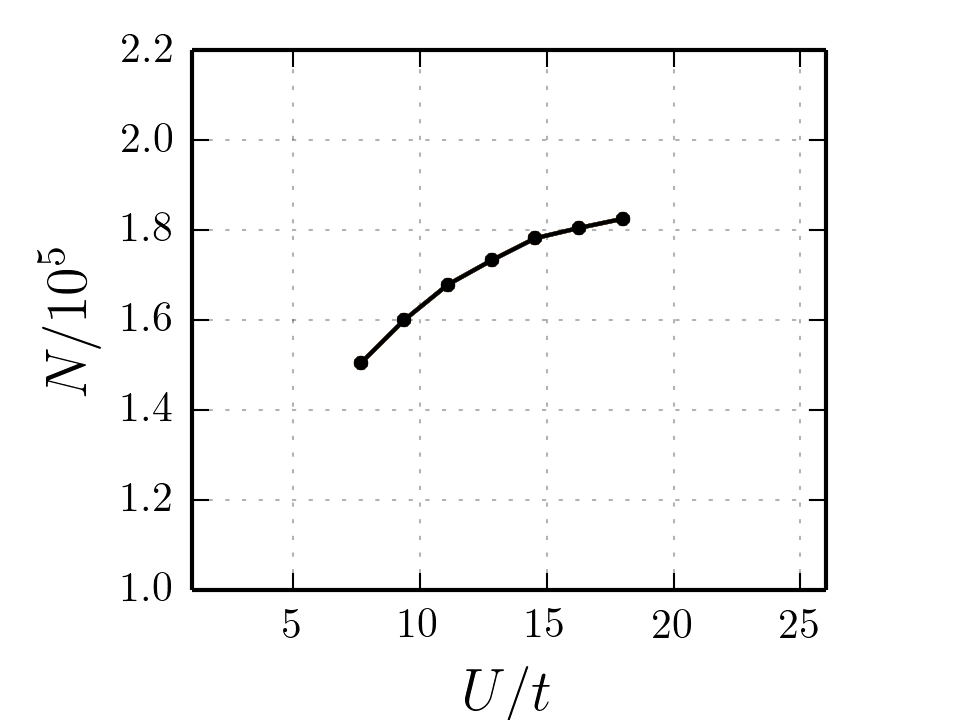
\includegraphics[width=0.5\textwidth]{figures/udataN.png}
\caption{$U/t$ and $N$ used to produce LDA results and compare to the
experimental data. } 
\label{fig:udataN}
\end{figure}

The comparison with experimental data is shown in Fig.~\ref{fig:udata}.  The
LDA curves are obtained for constant $T$.   In the last report we emphasized
that obtaining this results at constant entropy per particle $S/N$ would make
more sense,  so we were surprised by the fact the the LDA at constant $T$
agrees well with the data.   

\begin{figure}[H]
    \centering 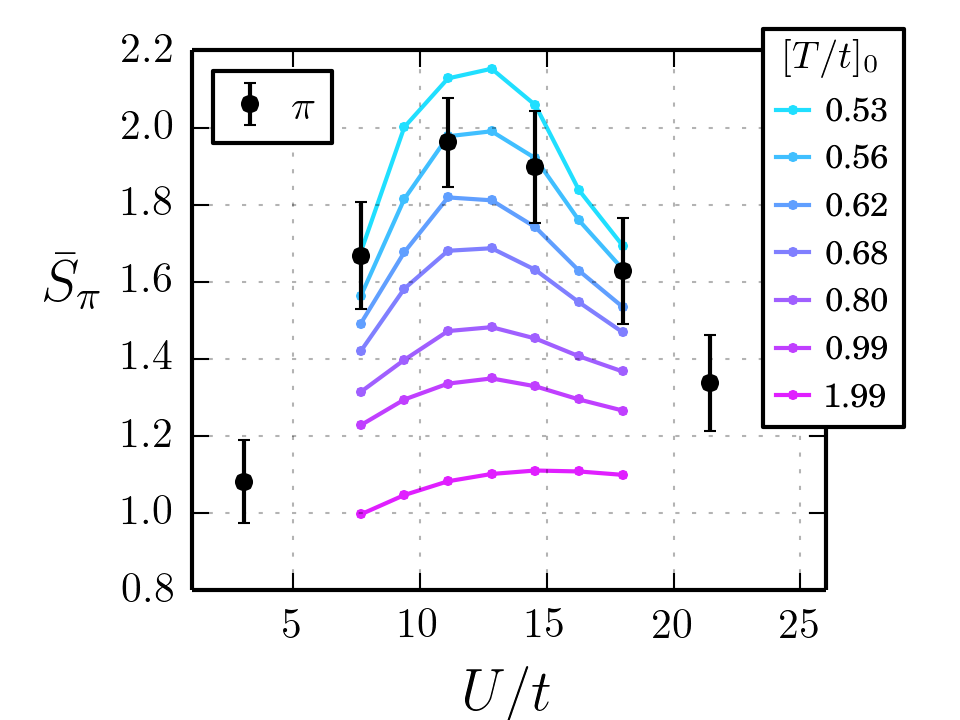
\includegraphics[width=0.6\textwidth]{figures/udata.png}
\caption{ Experimental data alongside LDA results.} 
\label{fig:udata}
\end{figure}


For the LDA points at which all of the necessary QMC entropy data is available,
we calculated the overall entropy to get an idea of what kind of entropy
variation we get at constant $T$ when varying $U/t$ and $N$ as we do here.  The
result is shown in Fig.~\ref{fig:udataS}.   What we see is that the slope of
this $S/N$ curves is not too large,  so for our data the difference between
constant $T$ and constant $S/N$ is going to be small and perhaps negligible.  

\begin{figure}[H]
    \centering 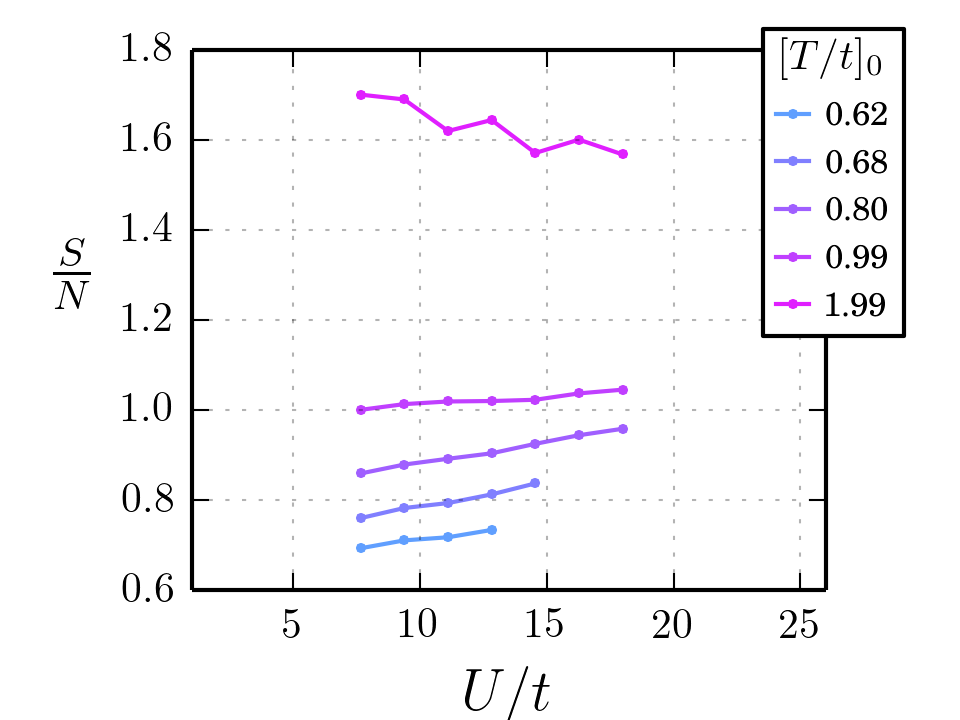
\includegraphics[width=0.5\textwidth]{figures/udataS.png}
\caption{ Overall entropy per particle $S/N$ for LDA results.} 
\label{fig:udataS}
\end{figure}


Finally, please notice that in the plots shown in this report we are using
$[T/t]_{0}$, which is the local value of $T/t$ at the center of the trap.   We
could also use $[T/t]^{*}$, which is the local value of $T/t$ at the radius at
which $S_{\pi}$ is maximized.  
 
\bibliographystyle{osa} \bibliography{latt_evap}

\end{document}




